%%%%%%%%%%%%%%%%%%%%%%%%% 
%% SITE A GARDER : http://titilog.free.fr/


\documentclass[10pt]{beamer}
% \includeonlyframes{yy}
\usepackage[english]{babel}
\usepackage{color, colortbl}
\definecolor{Gray}{gray}{0.9}
\newcolumntype{g}{>{\columncolor{Gray}}c}
\hypersetup{%
  % pdfborder = {0 0 0},
  colorlinks, urlcolor=blue, linkcolor=, }

\makeatletter \let\@mycite\@cite
\def\@cite#1#2{{\hypersetup{linkcolor=mLightBlue}[{#1\if@tempswa ,
      #2\fi}]}} \makeatother

\usetheme{m} %%%%%
% \usepackage[version=3]{mhchem}
\usepackage{caption}
\captionsetup[figure]{labelformat=empty}
\usepackage{fontspec}
\usepackage{xcolor}
\usepackage{siunitx}
% \usepackage[backend=bibtex]{biblatex} \usepackage[square]{natbib}
% \bibliography{main}
\usepackage[]{algorithm2e}
\usefonttheme[onlymath]{serif} \usepackage{amsmath}
\usepackage{subcaption} \usepackage{appendixnumberbeamer}
\usepackage{tabularx, booktabs} \usepackage{multirow}
\usepackage{multicol} \usepackage{array} \usepackage{pbox}
\usepackage{mathtools}
\usepackage{adjustbox}
\definecolor{darkred}{HTML}{D38989}
\definecolor{darkgreen}{HTML}{66D191}
\PassOptionsToPackage{enumerate}{shortlabels} \newcommand\ExtraSep
{\dimexpr\cmidrulewidth\relax}
\captionsetup{font=scriptsize,labelfont=scriptsize}
% \addtobeamertemplate{background canvas}{\transfade[duration=0.05]}{}


\title{Fusion of Three-Dimensional Mass Spectrometry and Magnetic Resonance Images}
\subtitle{\normalsize Application to the wheat grain}
\institute{OurCon 2021}
\author{{Florent \textsc{Grélard}\\
    David \textsc{Legland}, Mathieu \textsc{Fanuel}, Loïc \textsc{Foucat}, Hélène \textsc{Rogniaux}}}
\titlegraphic{\hspace*{0.01\textwidth}~%
  
\includegraphics[width=0.2\textwidth]{fig/logo-inrae}\hspace*{0.075\textwidth}~%
  
\includegraphics[width=0.2\textwidth]{fig/logo-bibs.png}\hspace*{0.075\textwidth}~%
  
\includegraphics[width=0.2\textwidth]{fig/logo-biogenouest}\hspace*{0.075\textwidth}~%
  
\includegraphics[width=0.2\textwidth]{fig/logo-region}\hspace*{0.01\textwidth}~%
} \setbeamercolor{bbb}{fg=red}

\let\oldfootnotesize\footnotesize
\renewcommand*{\footnotesize}{\oldfootnotesize\tiny}
\newcommand\labelitemi{$\bullet$}
\renewcommand{\thefootnote}{[\arabic{footnote}]}
% \newrobustcmd*{\footlessfullcite}{\AtNextCite{\renewbibmacro{in:}{}\renewbibmacro{year:}{}}\footfullcite}
% \newrobustcmd*{\lessfullcite}{\AtNextCite{\renewbibmacro{in:}{}\renewbibmacro{year:}{}}\fullcite}

\newcommand{\cfbox}[2]{%
    \colorlet{currentcolor}{.}%
    {\color{#1}%
    \fbox{\color{currentcolor}#2}}%
}


\newcommand{\backupbegin}{ \newcounter{framenumberappendix}
  \setcounter{framenumberappendix}{\value{framenumber}} }
\newcommand{\backupend}{
  \addtocounter{framenumberappendix}{-\value{framenumber}}
  \addtocounter{framenumber}{\value{framenumberappendix}} }
% http://mcclinews.free.fr/latex/introbeamer/les_couleurs.html
\begin{document}

% affiche le logo en bas à droite
% \logo{
\includegraphics[height=0.5cm]{fig/logo-inra}}
% enlève la barre de navigation
\setbeamertemplate{navigation symbols}{ }
\setbeamertemplate{blocks}[rounded][shadow=false]
% Ombre aux blocks
\setbeamertemplate{caption}{\insertcaption}

\date{\vspace{0.2cm}13 October 2021} % set the Date
% \renewcommand{\insertnavigation}[1]{}

% \AtBeginSection[]{

% }

% \institute{INRAE de Nantes}
\makeatletter
\AtBeginPart{%
  \beamer@tocsectionnumber=0\relax
  \setcounter{section}{0}
}
\makeatother

\begin{frame}[plain]
  \titlepage
\end{frame}

\section{Context}
\begin{frame}{Wheat grain}
  Study of \textbf{wheat grain development}.

  \begin{figure}[ht]
    \centering
    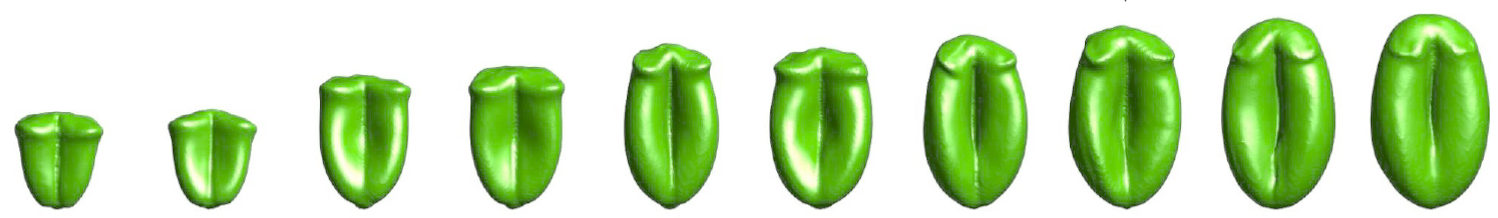
\includegraphics[width=0.9\textwidth]{fig/stages}
  \end{figure}

  
  \textbf{Cell walls}:
  \begin{itemize}
  \item specific mechanical properties for growth.
  \item layered polymers involving \textbf{celluloses}, \textbf{hemicelluloses}.
  \end{itemize}

  

\end{frame}

\begin{frame}{Arabinoxylans and water transfers}

  \alert{Arabinoxylans (AX)}: cell wall polysaccharides.
  \vspace{-0.2cm}
  \begin{figure}[ht]
    \centering
    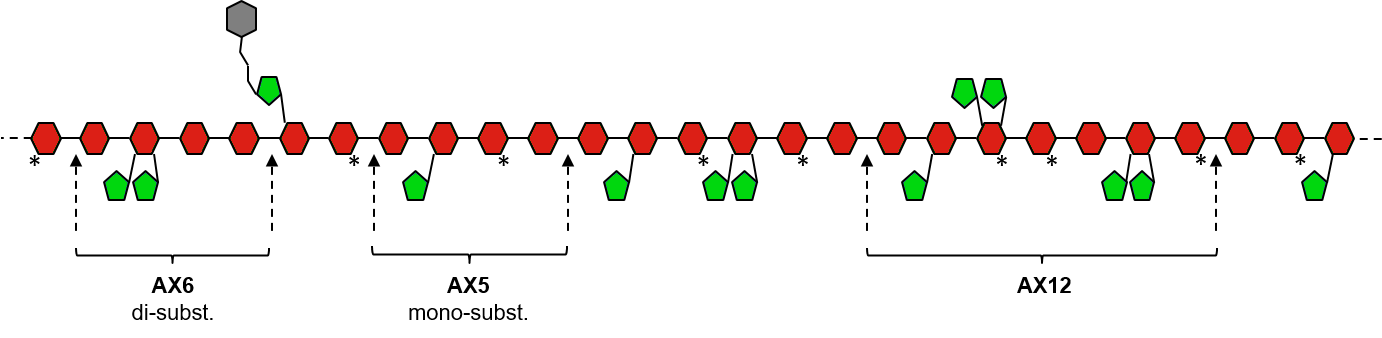
\includegraphics[width=0.9\textwidth]{fig/AX}
  \end{figure}


 
  

  \begin{columns}[totalwidth=\textwidth]
    \begin{column}[t]{0.5\linewidth}
        {AX localized in \textbf{highly hydrated} regions \cite{Fanuel18}:}
    \end{column}
    \begin{column}[c]{0.5\linewidth}
      \hfill
      \begin{figure}[ht]
        \centering
        \begin{subfigure}[t]{0.45\textwidth}
          \centering
          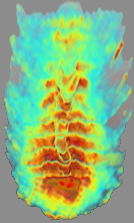
\includegraphics[width=0.6\textwidth]{fig/3DAX}
          \label{subfig:3Darabinoxylan}
        \end{subfigure}%
        \begin{subfigure}[t]{0.45\textwidth}
          \centering
          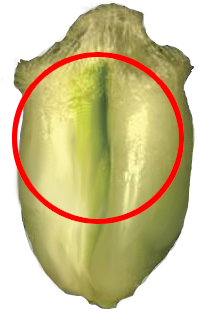
\includegraphics[width=0.6\textwidth]{fig/water_transfer}
          \label{subfig:water_transfer}
        \end{subfigure}%
      \end{figure}
    \end{column}
  \end{columns}
  

     \underline{Aim:} to identify \textbf{new molecules} whose spatial distribution correlate with water.\\

   \end{frame}


\begin{frame}{From images to molecule identification}
  \textbf{(a)} \textbf{IRM :} images enclosing the water distribution
   \vspace{0.1cm}

  \textbf{(b)} \textbf{MSI (MALDI):} hyperspectral image: spectrum associated to each pixel location.

  $\rightarrow$ Automatic image \alert{fusion}

  \underline{Problem:} differences between imaging modalities and resulting images.

  \vspace{-0.2cm}
  \begin{figure}[ht]
    \centering
    \begin{subfigure}[t]{0.4\textwidth}
      \centering 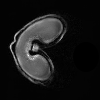
\includegraphics[width=0.65\textwidth]{fig/mri_slice11}
      \caption{}
      \label{subfig:mri}
    \end{subfigure}%
    \begin{subfigure}[t]{0.4\textwidth}
      \centering 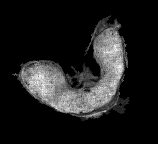
\includegraphics[width=0.7\textwidth]{fig/maldi}
      \caption{}
      \label{subfig:maldi}
    \end{subfigure}%
    \label{fig:irm_vs_maldi}
  \end{figure}
  
\end{frame}

\begin{frame}{MR and MS imaging}

  \underline{\textbf{MRI:}} \hspace{0.5\textwidth} \underline{\textbf{MSI} (MALDI--TOF):}

  \begin{columns}
    \begin{column}[t]{.5\textwidth}
      \begin{itemize}
      \item \textbf{Whole} grain
      \item \textbf{4D images}:  \alert{multi-pulse} sequence (gradient echo)
      \item \textbf{Resolution}: $50 \mu m \times 50 \mu m \times 500 \mu m$
      \end{itemize}
      \vspace{1cm}
      \begin{figure}[ht]
        \centering
        \begin{subfigure}[t]{0.33\textwidth}
          \centering 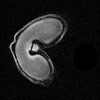
\includegraphics[width=0.9\textwidth]{fig/echo2_1}
        \end{subfigure}%
        \begin{subfigure}[t]{0.33\textwidth}
          \centering 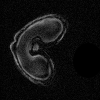
\includegraphics[width=0.9\textwidth]{fig/echo2_2}
        \end{subfigure}%
        \begin{subfigure}[t]{0.33\textwidth}
          \centering 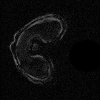
\includegraphics[width=0.9\textwidth]{fig/echo2_3}
        \end{subfigure}%
      \end{figure}
    \end{column}
    \begin{column}[t]{.5\textwidth}
      \begin{itemize}
      \item \textbf{Sample preparation}: cut, enzymatic digestion, matrix spraying
      \item \textbf{Datacube}: spectral dimension (m/z ratios)
      \item \textbf{Resolution}: $25 \mu m \times 25 \mu m \times 80 \mu m$
      \end{itemize}
      \begin{figure}[ht]
        \centering
        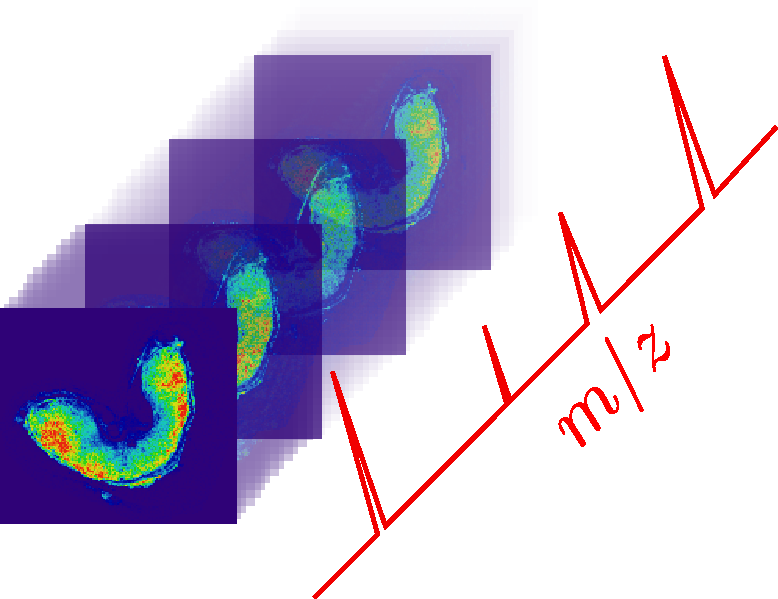
\includegraphics[width=0.5\linewidth]{fig/maldi_cube}
      \end{figure}
    \end{column}
  \end{columns}
\end{frame}


% \begin{frame}{Workflow in 2D}

%   Joint analysis of \textbf{water} distribution (MRI) with \textbf{individual molecules} (MSI).

%   Previously described workflow \textbf{in 2D} \cite{Grelard_2021}.


%   \begin{figure}[ht]
%     \centering
%     \includegraphics<1>[width=0.5\textwidth]{fig/maldi_corr1}%
%     \includegraphics<2->[width=0.5\textwidth]{fig/maldi_corr2}%
%   \end{figure}

%   \visible<3->{

%     $\Rightarrow$ \textbf{mathematical} and \textbf{computational} methods: signal and image processing, statistical analysis.
  
%   }
% \end{frame}



\begin{frame}{3D data}
  Wheat grain from the \textbf{Bobwhite} variety, 3 stages of development.
  
  \underline{Problem:}
  \begin{itemize}
  \item intensity inhomogeneities
  \item different orientations
  \end{itemize}


   \begin{figure}[ht]
  \centering
  \begin{subfigure}[t]{0.5\textwidth}
    \centering
    \includegraphics<1>[width=0.65\textwidth]{fig/3D_density_aligned_manual0000}%
    \includegraphics<2>[width=0.65\textwidth]{fig/3D_density_aligned_manual0003}%
    \includegraphics<3>[width=0.65\textwidth]{fig/3D_density_aligned_manual0006}%
    \includegraphics<4->[width=0.65\textwidth]{fig/3D_density_aligned_manual0009}
  \end{subfigure}%
    \begin{subfigure}[t]{0.5\textwidth}
    \centering
    \includegraphics<1>[width=0.65\textwidth]{fig/3D_segmentation0000}%
    \includegraphics<2>[width=0.65\textwidth]{fig/3D_segmentation0003}%
    \includegraphics<3>[width=0.65\textwidth]{fig/3D_segmentation0006}%
    \includegraphics<4->[width=0.65\textwidth]{fig/3D_segmentation0009}
  \end{subfigure}%
\end{figure}

\visible<5> {
  $\Rightarrow$ need for \textbf{reproducible} and
  \textbf{generic} computational methods.
}




    
\end{frame}


%\ begingroup \setbeamercolor{background
%     canvas}{bg=mLightBlue}
  
%   \setbeamertemplate{subsection in toc}
%   {\leavevmode\leftskip=2em$\bullet$\hskip1em\inserttocsubsection\par}
%   \setbeamercolor{section in toc}{fg=paleGrey, bg=mLightBlue}
%   \setbeamercolor{local structure}{fg=mLightBlueLighter,bg=mLightBlue}
%   \setbeamercolor{section in toc shaded}{fg=mLightBlue, bg=mLightBlue}
%   \setbeamertemplate{section in toc}[circle]
%   \setbeamertemplate{section in toc shaded}[default][80]
%   \setbeamertemplate{section in toc}{\hspace*{1em}\inserttocsection}

%   \setbeamercolor{subsection in toc}{fg=paleGrey, bg=mLightBlue}
%   \begin{frame}[noframenumbering,plain]
%     \frametitle{\textcolor{paleGrey}{Table des matières}}

%     \tableofcontents[currentsection, sectionstyle=show/hide,
%     hideothersubsections]
%   \end{frame}
%   \endgroup }



\AtBeginSection[]{
  \begingroup
  \setbeamercolor{background canvas}{bg=mLightBlue}

  \setbeamertemplate{subsection in toc}
  {\leavevmode\leftskip=2em$\bullet$\hskip1em\inserttocsubsection\par}

  % \setbeamercolor{section in toc shaded}{bg=paleGrey}


  \setbeamercolor{section in toc}{fg=paleGrey, bg=mLightBlue}
  \setbeamercolor{local structure}{fg=mLightBlueLighter,bg=mLightBlue}
  \setbeamercolor{section in toc shaded}{fg=mLightBlue, bg=mLightBlue}
  \setbeamertemplate{section in toc}[circle] \setbeamertemplate{section
    in toc shaded}[default][80]
    \setbeamertemplate{section in toc}{\hspace*{1em}\inserttocsection}



  \setbeamercolor{subsection in toc}{fg=paleGrey, bg=mLightBlue}
  \begin{frame}[plain,noframenumbering]
      \frametitle{\textcolor{paleGrey}{Contents}}
      \tableofcontents[currentsection, hideothersubsections]
    \end{frame}
    \endgroup
}
\section{3D workflow}
\begin{frame}{3D workflow}

  Extension of our \textbf{2D} workflow \cite{Grelard_2021}.
  \begin{enumerate}
  \item<2-> \textbf{3D registration}
  \item<3-> Spatial correlations with \textbf{uncertainties}
  \item<4-> \textbf{Visualization} of 3D MS images

  \end{enumerate}

  \begin{figure}[ht]
    \centering
    \includegraphics<1>[width=0.7\textwidth]{fig/workflow3D_0}%
    \includegraphics<2>[width=0.7\textwidth]{fig/workflow3D_2}%
    \includegraphics<3>[width=0.7\textwidth]{fig/workflow3D_3}%
    \includegraphics<4>[width=0.7\textwidth]{fig/workflow3D_4}%
  \end{figure}
\end{frame}


% \AtBeginSection[]{ \begingroup \setbeamercolor{background
%     canvas}{bg=mLightBlue}
  
%   \setbeamertemplate{subsection in toc}
%   {\leavevmode\leftskip=2em$\bullet$\hskip1em\inserttocsubsection\par}
%   \setbeamercolor{section in toc}{fg=paleGrey, bg=mLightBlue}
%   \setbeamercolor{local structure}{fg=mLightBlueLighter,bg=mLightBlue}
%   \setbeamercolor{section in toc shaded}{fg=mLightBlue, bg=mLightBlue}
%   \setbeamertemplate{section in toc}[circle]
%   \setbeamertemplate{section in toc shaded}[default][80]
%   \setbeamertemplate{section in toc}{\hspace*{1em}\inserttocsection}

%   \setbeamercolor{subsection in toc}{fg=paleGrey, bg=mLightBlue}
%   \begin{frame}[noframenumbering,plain]
%     \frametitle{\textcolor{paleGrey}{Table des matières}}

%     \tableofcontents[currentsection, sectionstyle=show/hide,
%     hideothersubsections]
%   \end{frame}
%   \endgroup }


% \section{Normalization of MS images}
% \begin{frame}{Normalization}

%   Normalization factors:
%   \begin{enumerate}
%   \item Total ion count (TIC): sum of spectra intensities
%   \item Intensity of a standard molecule
%   \item Median
%   \end{enumerate}

%   \vspace{0.2cm}

%   Usually, the \textbf{TIC} is used: compensates for differences in the detected signals.
% \end{frame}


% \begin{frame}{TIC: problem}
%   Intensity variation between two spectra $\Rightarrow$
%   different TIC factors.
  
%   \begin{figure}[ht]
%     \centering
%     \includegraphics<1>[width=0.7\textwidth]{fig/normalization1}%
%     \includegraphics<2>[width=0.7\textwidth]{fig/normalization2}%
%     \includegraphics<3>[width=0.7\textwidth]{fig/normalization3}%
%   \end{figure}

% \end{frame}

% \begin{frame}{TIC: problem}

%   \underline{Example:} high intensity of the insulin peak in mouse pancreas \cite{Deininger_2011}.

%   \begin{figure}[ht]
%     \centering
%     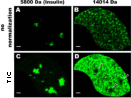
\includegraphics[width=0.7\textwidth]{fig/normalization_defect}
%     \caption{}
%     \label{fig:normalization_defect}
%   \end{figure}

% \end{frame}


% \begin{frame}{Noise Ion Count}

%   \textbf{Idea:} remove peak contribution from the normalization factor.

%   \textbf{Calcul:} NIC = TIC - $\sum I_{\text{peaks}}$

%   \vspace{0.4cm}

%   \begin{figure}[ht]
%     \centering
%     \includegraphics<1>[width=0.7\textwidth]{fig/normalization2}%
%     \includegraphics<2>[width=0.7\textwidth]{fig/normalization_sic1}%
%     \includegraphics<3>[width=0.7\textwidth]{fig/normalization_sic2}%
%     \includegraphics<4>[width=0.7\textwidth]{fig/normalization_sic3}%
%     \caption{}
%     \label{fig:normalization_sic1}
%   \end{figure}


% \end{frame}


% \section{3D Registration}

\begin{frame}{Registration}

  Registration methods defined by three components:
  \begin{enumerate}
  \item The \textbf{geometrical transformation}: rigid, affine, deformable
  \item The \textbf{metric}: estimates the similarity between the reference and target images, using intensity or geometrical criteria
  \item The \textbf{optimization}: to find the minimum of the metric \vspace{0.3cm}
  \end{enumerate}
  \vspace{-0.4cm}
  
   \begin{figure}[ht]
    \includegraphics<1>[width=0.6\textwidth]{fig/registration1}%
    \includegraphics<2>[width=0.6\textwidth]{fig/registration2}%
    \includegraphics<3>[width=0.6\textwidth]{fig/registration3}%
    \includegraphics<4>[width=0.6\textwidth]{fig/registration4}%
  \end{figure}

  

\end{frame}



\begin{frame}{Registration}

  \textbf{Problems:} intensity discrepancies, different orientations

   \begin{figure}[ht]
    \centering
    \begin{subfigure}[t]{0.5\textwidth}
      \centering
      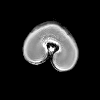
\includegraphics[width=0.65\textwidth]{fig/mri_slice6.png}
    \end{subfigure}%
    \begin{subfigure}[t]{0.5\textwidth}
      \centering
      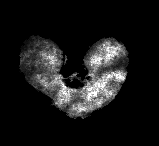
\includegraphics[width=0.65\textwidth]{fig/maldi_slice6}
    \end{subfigure}%

  \end{figure}

  \onslide<2->{
  $\Rightarrow$ Hard to choose  \textbf{appropriate parameters} in order to register all slices.
  }
 

\end{frame}

\begin{frame}{Registration approach}
  
  Two steps:
  \begin{enumerate}
  \item \textbf{2D exhaustive} affine registration
  \item \textbf{3D deformable} registration
  \end{enumerate}

  \alert{Exhaustive registration}: \textbf{predefined} transformation parameters  $\Rightarrow$ avoids converging towards a \textbf{local minimum}.

  \begin{figure}[ht]
    \centering
    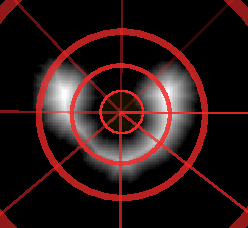
\includegraphics[width=0.4\textwidth]{fig/exhaustive_registration}
    \caption{}
    \label{fig:exhaustive_registration}
  \end{figure}

  
\end{frame}

\begin{frame}{Similarity metric}

  Geometrical metric: \textbf{distance transform} (DT)

  \alert{Distance transform}: maps each pixel of an object to its distance to the border.

  \begin{figure}[ht]
    \centering
    \begin{subfigure}[t]{0.5\textwidth}
      \centering
      \includegraphics<1>[width=0.65\textwidth]{fig/mri_slice6.png}%
      \includegraphics<2>[width=0.65\textwidth]{fig/mri_slice6_dt.png}
      \caption{}
      \label{subfig:mri_slice6_dt.png}
    \end{subfigure}%
    \begin{subfigure}[t]{0.5\textwidth}
      \centering
      \includegraphics<1>[width=0.65\textwidth]{fig/maldi_slice6.png}%
      \includegraphics<2>[width=0.65\textwidth]{fig/maldi_slice6_dt.png}
      \caption{}
      \label{subfig:maldi_slice6_dt.png}
    \end{subfigure}%
  \end{figure}

  
\end{frame}

\begin{frame}{Exhaustive registration}

  Transformation initialized by aligning the centers of mass of the shapes.

  \begin{itemize}
  \item Transformation: parameter space for rotation and scaling
  \item Metric: Mutual information on the \textbf{DT of the object}
  \item Optimization: \textbf{exhaustive}
  \end{itemize}

  \vspace{-0.2cm}
  \begin{figure}[ht]
    \centering
    \includegraphics<1>[width=0.65\textwidth]{fig/metric_exh_0}%
    \includegraphics<2>[width=0.65\textwidth]{fig/metric_exh_1}%
    \includegraphics<3>[width=0.65\textwidth]{fig/metric_exh_2}
    \label{fig:metric_2}
  \end{figure}

\end{frame}

\begin{frame}{Deformable registration}
  Local deformations change distance transformation values.

  \vspace{0.4cm}
  
  \textbf{New metric}: sum of squared differences with an \textbf{update} on DT values.

  \begin{figure}[ht]
  \centering
  \begin{subfigure}[t]{0.2\textwidth}
    \centering
    
\includegraphics[width=0.95\textwidth]{fig/registration_reference}
    \caption{}
    \label{subfig:registration_reference}
  \end{subfigure}%
  \begin{subfigure}[t]{0.2\textwidth}
    \centering
    
\includegraphics[width=0.95\textwidth]{fig/registration_target}
    \caption{}
    \label{subfig:registration_target}
  \end{subfigure}%
  \begin{subfigure}[t]{0.2\textwidth}
    \centering
    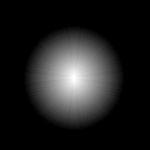
\includegraphics[width=0.95\textwidth]{fig/registration_reference_dt}
    \caption{}
    \label{subfig:registration_dt_reference}
  \end{subfigure}%
  \begin{subfigure}[t]{0.2\textwidth}
    \centering
    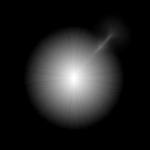
\includegraphics[width=0.95\textwidth]{fig/registration_target_dt_interpol.png}
    \caption{}
    \label{subfig:registration_dt_target_interpol}
  \end{subfigure}%
  \begin{subfigure}[t]{0.2\textwidth}
    \centering
    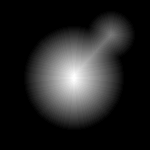
\includegraphics[width=0.95\textwidth]{fig/registration_target_dt}
    \caption{}
    \label{subfig:registration_dt_target}
  \end{subfigure}%
\end{figure}
\end{frame}


\begin{frame}{Deformable registration}
  
  \begin{columns}
    \begin{column}[t]{0.6\textwidth}
      \textbf{Variational methods}: displacements modelled by a \textbf{vector field}. The vector field is guided by pixel similarity. \vspace{0.2cm}

      \begin{enumerate}
      \item External forces: metric $\textcolor{red}{\mathcal{D}}$: sum of squared differences with DT update
      \item Internal forces: \textbf{regularization} term $\textcolor{blue}{\mathcal{S}}$
      \end{enumerate}

      \[
        \mathcal{J}[y] = \textcolor{red}{\mathcal{D}[\mathcal{T}[y], \mathcal{R}]} + \textcolor{blue}{\mathcal{S}[y]} \xrightarrow{y} \min
      \]
      
      % \[
      %   \mathcal{J}[y] = \textcolor{red}{\mathcal{D}[\mathcal{T}[y], \mathcal{R}]} + \textcolor{blue}{\mathcal{S}[y]} \xrightarrow{y} \min
      % \]
    \end{column}
    \begin{column}[t]{0.4\textwidth}
      \begin{figure}[ht]
        \centering
        \includegraphics<1>[width=0.95\textwidth]{fig/registration_nonrigid_vectorfield_2}%
        \includegraphics<2>[width=0.95\textwidth]{fig/registration_nonrigid_vectorfield_10}%
        \includegraphics<3>[width=0.95\textwidth]{fig/registration_nonrigid_vectorfield_30}%
        \includegraphics<4>[width=0.95\textwidth]{fig/registration_nonrigid_vectorfield}%
      \end{figure}
    \end{column}
  \end{columns}
\end{frame}




\begin{frame}{Statistical analysis}
  
  \begin{columns}
    \begin{column}[t]{0.6\textwidth}
      \begin{enumerate}
      \item Dimension reduction of the MS image by \textbf{NMF} 
      \item \textbf{Projection} of the MR image onto the NMF axes
      \item Selection of ion images which are \textbf{the closest} to the MR projection
      \end{enumerate}
    \end{column}
    \begin{column}[t]{0.4\textwidth}
      \begin{figure}[ht]
        \centering
        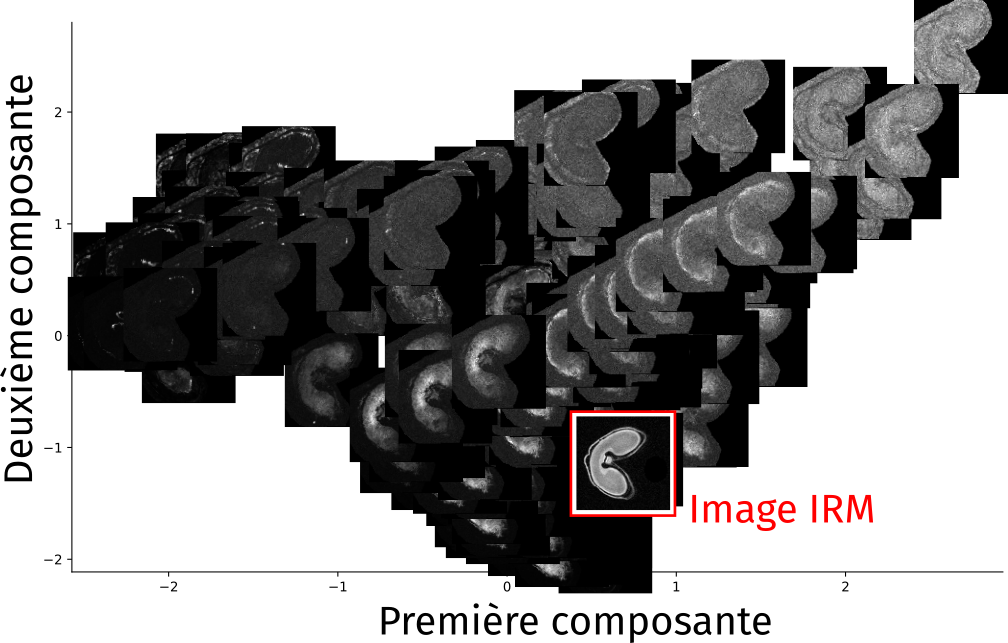
\includegraphics[width=0.95\textwidth]{fig/pca_big3}
      \end{figure}
    \end{column}
  \end{columns}
\end{frame}

\begin{frame}{Statistical analysis}
  Identification of molecules in MALDI which \textbf{correlate with MR images}:

  \textbf{Problem:} similar regions in both images might not be aligned.

  \begin{figure}[ht]
  \centering
  \begin{subfigure}[t]{0.33\textwidth}
    \centering
    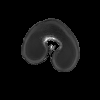
\includegraphics[width=0.9\textwidth]{fig/t2_6_original}
    \caption{}
    \label{subfig:t2_6_original}
  \end{subfigure}%
  \begin{subfigure}[t]{0.33\textwidth}
    \centering
    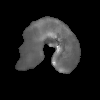
\includegraphics[width=0.9\textwidth]{fig/msi_6_original}
    \caption{}
    \label{subfig:msi_6_original}
  \end{subfigure}%
  \begin{subfigure}[t]{0.33\textwidth}
    \centering
    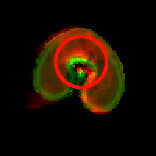
\includegraphics[width=0.9\textwidth]{fig/overlay_t2_6_original}
    \caption{}
    \label{subfig:overlay_t2_6_original}
  \end{subfigure}%
\end{figure}

\end{frame}


\begin{frame}{Statistical analysis}
  \textbf{Contribution:} exhaustive registration of individual NMF component images


  \begin{figure}[ht]
    \centering
    \includegraphics<1>[width=0.9\textwidth]{fig/translation_nmf_0}%
    \includegraphics<2>[width=0.9\textwidth]{fig/translation_nmf_1}%
    \includegraphics<3>[width=0.9\textwidth]{fig/translation_nmf_2}%
    \includegraphics<4>[width=0.9\textwidth]{fig/translation_nmf_3}%
  \end{figure}

  
\end{frame}







% \section{Visualization}

% \begin{frame}{Visualisation 3D}
  
%   3D volumetric rendering:
%   \begin{figure}[ht]
%     \centering
%     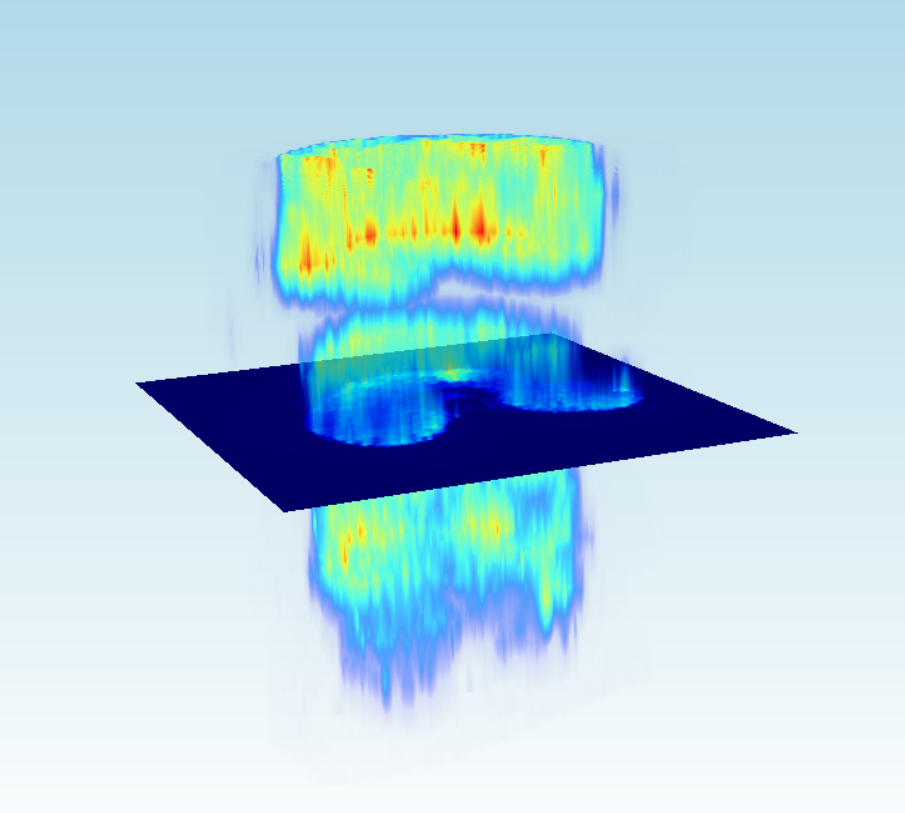
\includegraphics[width=0.5\textwidth]{fig/visu_3d.png}
%     \caption{}
%     \label{fig:visu_3d.png}
%   \end{figure}

% \end{frame}

\section{Results}

\begin{frame}{Registration}

  \vspace{-0.3cm}
  Percentage of shared pixels between the MS and MR images:
  \begin{itemize}
  \item \textbf{simple} with a intensity-based metric: \textbf{77.9\%}
  \item \textbf{(b)} \textbf{exhaustive} with DT: \textbf{84.6\%}
  \item \textbf{(c)} \textbf{variational} without DT update: \textbf{90.2\%}
  \item \textbf{(d)} \textbf{variational} with DT update: \textbf{93.2\%}
  \end{itemize}

  \begin{figure}[ht]
  \centering
  \begin{subfigure}[t]{0.25\textwidth}
    \centering
    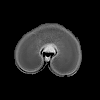
\includegraphics[width=0.95\textwidth]{fig/registration_wheat_mri}
    \caption{}
    \label{subfig:registration_wheat_mri}
  \end{subfigure}%
  \begin{subfigure}[t]{0.25\textwidth}
    \centering
    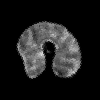
\includegraphics[width=0.95\textwidth]{fig/registration_wheat_affine}
    \caption{}
    \label{subfig:registration_wheat_affine}
  \end{subfigure}%
  \begin{subfigure}[t]{0.25\textwidth}
    \centering
    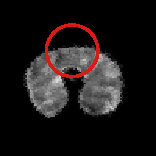
\includegraphics[width=0.95\textwidth]{fig/registration_wheat_ssd}
    \caption{}
    \label{subfig:registration_wheat_ssd}
  \end{subfigure}%
  \begin{subfigure}[t]{0.25\textwidth}
    \centering
    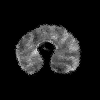
\includegraphics[width=0.95\textwidth]{fig/registration_wheat_dtssd}
    \caption{}
    \label{subfig:registration_wheat_dtssd}
  \end{subfigure}%
\end{figure}
\end{frame}

\begin{frame}{Statistical analysis}
  Mean squared error of the standard deviation between the \textbf{(a)} original and the \textbf{(b-c)} projected MR images:
  \begin{itemize}
  \item \textbf{without} NMF component image registration: \textbf{12.4}
  \item \textbf{with} NMF component image registration: \textbf{11.5}
  \end{itemize}

    \begin{figure}[ht]
  \centering
  \begin{subfigure}[t]{0.3\textwidth}
    \centering
    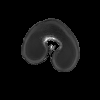
\includegraphics[width=0.95\textwidth]{fig/t2_6_original}
    \caption{}
    \label{subfig:t2_6_original}
  \end{subfigure}%
  \begin{subfigure}[t]{0.3\textwidth}
    \centering
    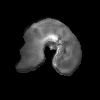
\includegraphics[width=0.95\textwidth]{fig/reconstruction_t2_translated.png}
    \caption{}
    \label{subfig:reconstruction_t2_translated.png}
  \end{subfigure}%
    \begin{subfigure}[t]{0.3\textwidth}
    \centering
    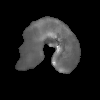
\includegraphics[width=0.95\textwidth]{fig/msi_6_original.png}
    \caption{}
    \label{subfig:reconstruction_t2_translated.png}
  \end{subfigure}%
\end{figure}

\end{frame}

\begin{frame}{Correlative analysis}

  Results on the \textbf{Bobwhite} wheat grain variety (250 DAA stage):

    \begin{figure}[ht]
    \centering
    \begin{subfigure}[t]{0.33\textwidth}
      \centering
      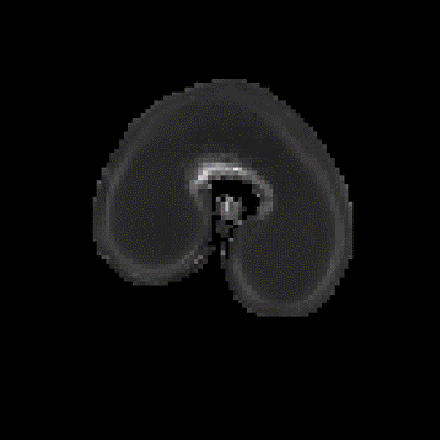
\includegraphics[width=0.9\textwidth]{fig/mri_slice8_250}
      \caption{$T_2^*$ MR image}
      \label{subfig:mri_slice8_250}
    \end{subfigure}%
    \begin{subfigure}[t]{0.33\textwidth}
      \centering
      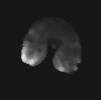
\includegraphics[width=0.9\textwidth]{fig/ax14_4ac}
      \caption{AX14.4Ac}
      \label{subfig:zonetir_0}
    \end{subfigure}%
    \begin{subfigure}[t]{0.33\textwidth}
      \centering
      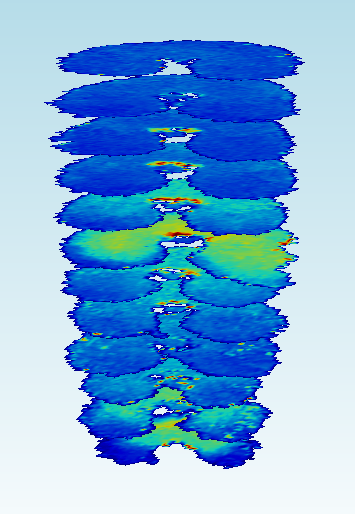
\includegraphics[width=0.7\textwidth]{fig/3D_250DJ}
      \caption{$\dfrac{\text{AX6}}{\text{AX5}}$ (in 3D)}
      \label{subfig:3D_250DJ}
    \end{subfigure}%

  \end{figure}

  Distribution similar to that of water:
  \begin{itemize}
  \item AX with a high number of \textbf{acetyl groups}.
  \item $\frac{\text{AX6}}{\text{AX5}}$ ratio
  \end{itemize}


\end{frame}



\section{Conclusion}

\begin{frame}{Conclusion}

  Workflow suited for 3D MS image with \textbf{homogeneous or inhomogeneous intensities}.

  Results at the 250 DAA stage confirm \textbf{previous results}.

  \textbf{Esmraldi}: tools for the fusion of 3D MS images\footnote{\url{https://github.com/fgrelard/Esmraldi}}.


  \vspace{0.4cm}

  Prospects:
  \begin{itemize}
  \item \textbf{Full 3D} statistical analysis.
  \item Registration with \textbf{local scale variations}.
  \end{itemize}


\end{frame}

\section{}
\begin{frame}[plain]{Acknowledgments}
  \begin{figure}[ht]
      \centering
      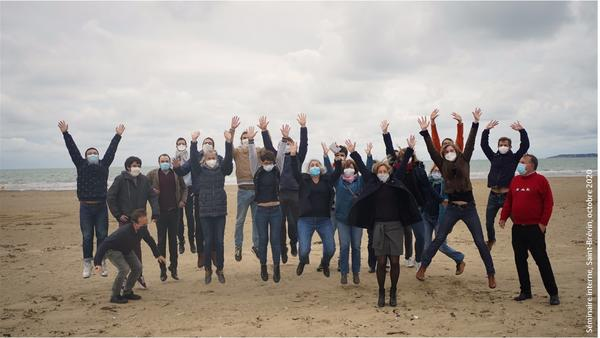
\includegraphics[width=0.7\textwidth]{fig/photoequipe}
    \end{figure}
    
    {\scriptsize
  \begin{itemize}
  \item \textbf{BIBS platform} : David Legland, Mathieu Fanuel, Loïc Foucat, Hélène Rogniaux
  \item \textbf{Former members}: Bastien Arnaud
  \item \textbf{Cell Walls team}: Luc Saulnier, Fabienne Guillon, Camille Alvarado, Anne--Laure Chateigner--Boutin
  \end{itemize}
}
\vspace{-0.5cm}
  \hspace*{0.01\textwidth}~%
  
\includegraphics[width=0.2\textwidth]{fig/logo-inrae}\hspace*{0.075\textwidth}~%
  
\includegraphics[width=0.2\textwidth]{fig/logo-bibs.png}\hspace*{0.075\textwidth}~%
  
\includegraphics[width=0.2\textwidth]{fig/logo-biogenouest}\hspace*{0.075\textwidth}~%
  
\includegraphics[width=0.2\textwidth]{fig/logo-region}\hspace*{0.01\textwidth}~%

\end{frame}




% \begin{frame}{Local scale variations}

%   \visible<2->{
%     The distance transform values are dependent on the local scale of the object.
%     }

%   \visible<3->{
%     \textbf{Idea:} normalize the DT values by the \textbf{local scale} of the object, taken as e.g. the object's radius.
%   }
  

%   \begin{figure}[ht]
%     \flushleft
%     \begin{subfigure}[t]{0.2\textwidth}
%       \centering
%       
\includegraphics[width=0.95\textwidth]{fig/prospect_reference}
%       \caption{}
%       \label{subfig:prospect_reference}
%     \end{subfigure}%
%     \begin{subfigure}[t]{0.2\textwidth}
%       \centering
%       
\includegraphics[width=0.95\textwidth]{fig/prospect_target}
%       \caption{}
%       \label{subfig:prospect_target}
%     \end{subfigure}%
%     \only<2->{%
%     \begin{subfigure}[t]{0.2\textwidth}
%       \centering
%       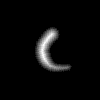
\includegraphics[width=0.95\textwidth]{fig/prospect_registered_target}
%       \caption{}
%       \label{subfig:prospect_registered_target}
%     \end{subfigure}%
%     }%
%     \only<3->{%
%       \begin{subfigure}[t]{0.2\textwidth}
%         \centering
%         
\includegraphics[width=0.95\textwidth]{fig/prospect_normalized_dt}
%         \caption{}
%         \label{subfig:prospect_normalized_dt}
%       \end{subfigure}%
%     }%
%     \only<4->{%
%       \begin{subfigure}[t]{0.2\textwidth}
%         \centering
%         
\includegraphics[width=0.95\textwidth]{fig/prospect_registered_target_normalized}
%         \caption{}
%         \label{subfig:prospect_registered_target_normalized}
%       \end{subfigure}%
%     }
%   \end{figure}

% \end{frame}






\appendix
\setbeamertemplate{headline}{%
  % \nointerlineskip
  % \begin{beamercolorbox}[wd=\paperwidth,leftskip=0.5cm,ht=0pt,dp=0pt]{block title}%
  %   \usebeamerfont{page number in head/foot}{\insertsection}
  % \end{beamercolorbox}%
  % \if@useTitleProgressBar
  % \nointerlineskip
  % % \vspace{-0.7cm}
  % \begin{beamercolorbox}[wd=\paperwidth,ht=0pt,dp=5pt]{section}
  %   \progressbar@titleprogressbar
  % \end{beamercolorbox}
  % \fi
  % \nointerlineskip
}

% \setbeamertemplate{frametitle}{%
%   \begin{beamercolorbox}[wd=\paperwidth,leftskip=0.7cm,rightskip=0.3cm,ht=0pt,dp=0pt]{frametitle}
%     \usebeamerfont{frametitle}\MakeLowercase{\protect\insertframetitle}
%   \end{beamercolorbox}
% }

\begin{frame}[allowframebreaks]
  \frametitle{Références}
  \setbeamertemplate{bibliography item}{$\bullet$}
  \bibliographystyle{apalike}
  \scriptsize{
    \bibliography{main}
  }
\end{frame}



\end{document}
